\begin{slide}{Program and Cast}
\begin{description}
\item[ACT I ({\em Warming Up}):] \hspace{1in} \\
\begin{itemize}
\item Introduction and Soot Basics {\blue (Laurie)}
\item Intraprocedural Analysis in Soot {\blue (Patrick)}
\end{itemize}
\item[ACT II ({\em The Home Stretch}):] \hspace{1in} \\
\begin{itemize}
\item Interprocedural Analyses and Call Graphs {\blue (Ond\v{r}ej)}
\item Attributes in Soot and Eclipse {\blue (Ond\v{r}ej,Feng,Jennifer)}
\item Conclusion, Further Reading \& Homework {\blue (Laurie)}
\end{itemize}
\end{description}
\end{slide}

\begin{slide}{Introduction and Soot Basics}
\begin{itemize}
\item What is Soot?
\item Soot: Past and Present
\item Soot Overview
\item IRs: Baf, {\red Jimple}, Shimple, Grimp, Dava
\item Soot as an end-user tool and Soot as an Eclipse plugin
\end{itemize}
\begin{center}
\textit{ ... switching gears .... }
\end{center}
\begin{itemize}
\item Jimple and Soot Implementation Basics 
\end{itemize}
\end{slide}

\begin{slide}{What is Soot?}
\begin{itemize}
\item a free compiler infrastructure, written in Java (LGPL)
\item was originally designed to analyze and transform Java bytecode
\item original motivation was to provide a common infrastructure with
which researchers could compare analyses (points-to analyses)
\item has been extended to include decompilation and visualization
\end{itemize}
\sablefootnote{www.sable.mcgill.ca/soot/}
\end{slide}

\begin{slide}{What is Soot?  (2)}
\begin{itemize}
\item Soot has many potential applications:
\begin{itemize}
  \item used as a stand-alone tool (command line or Eclipse plugin)
  \item extended to include new IRs, analyses, transformations and 
        visualizations
  \item as the basis of building new special-purpose tools 
\end{itemize}
\end{itemize}
\end{slide}

\begin{slide}{Soot: Past and Present}
\begin{itemize}
\item Started in 1996-97 with the development of \texttt{coffi} by
Clark Verbrugge and some first prototypes of \texttt{Jimple} IR by
Clark and Raja Vall\'ee-Rai.
\item First publicly-available versions of Soot 1.x were associated 
with Raja's M.Sc. thesis
\item New contributions and releases have been added by many
graduate students at McGill and research results have been the topics
of papers and theses.
\end{itemize}
\sablefootnote{www.sable.mcgill.ca/soot/credits}
\sablefootnote{www.sable.mcgill.ca/publications/}
\end{slide}

\begin{slide}{Soot: Past and Present (2)}

\begin{itemize}
\item Soot 1.x has been used by many research groups for 
a wide variety of applications.   Has also been used in several
compiler courses.  Last version was 1.2.5.
\item Soot 2.0 and the first version of the Eclipse Plugin have just
been released - June 2003 - JIT for PLDI 2003.
\item This tutorial is based on Soot 2.0. 
\end{itemize}
\end{slide}

\begin{slide}{Soot Overview}
\vspace{-.3in}
\begin{center}
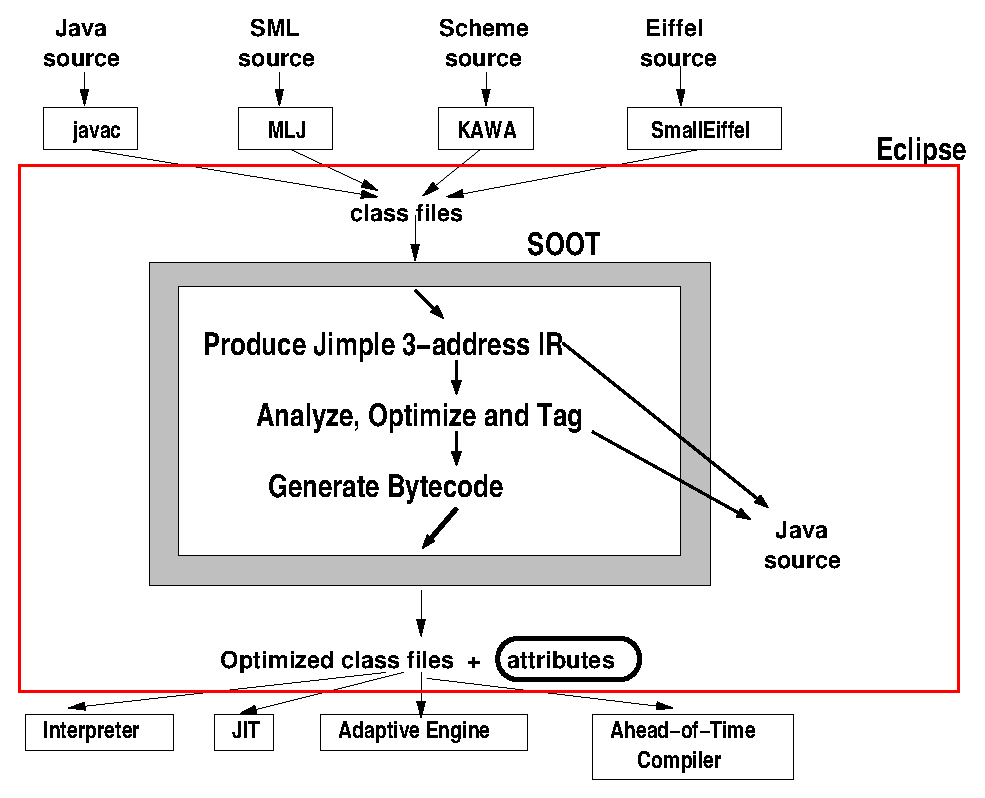
\epsfig{file=overview1.eps,width=3.9in}
\end{center}
\end{slide}

\begin{slide}{Soot IRs}
\begin{description}
\item[Baf:] is a compact rep. of {\red B}ytecode (stack-based)
\item[Jimple:]  is {\red J}ava's s{\red imple}, typed,  3-addr (stackless) representation 
\item[Shimple:]  is a {\red S}SA-version of {\red Jimple}
\item[Grimp:] is like J{\red imp}le, but with expressions ag{\red GR}egated 
\item[Dava:] structured representation used for {\red D}ecompiling J{\red ava}
\end{description}
\end{slide}

\begin{slide}{Soot as an end-user tool: Command-line}
\begin{enumerate}
\item Install Java.
\item Download two .jar files and put them on your CLASSPATH.
\end{enumerate}
\begin{description}
\item[\texttt{java soot.Main --help}] \hspace{1in} \\
 List options.
\item[\texttt{java soot.Main --version}] \hspace{1in} \\
 Print version information.
\end{description}
\sablefootnote{www.sable.mcgill.ca/software/\#soot}
\end{slide}

\begin{slide}{Command-line: processing classes}
\begin{description}
\item[\texttt{java soot.Main Foo}] \hspace{1in} \\   
 Process \texttt{Foo.class} in the current directory
 and produce a new class file in
\texttt{sootOutput/Foo.class}.
\item[\texttt{java soot.Main -f jimple Foo}] \hspace{1in} \\
Same as above, but produce Jimple in  \texttt{sootOutput/Foo.jimple}.
\item[\texttt{java soot.Main -f dava Foo}] \hspace{1in} \\
Decompile \texttt{Foo.class} and produce \texttt{Foo.java} in 
\texttt{sootOutput/dava/src/Foo.java}.
\end{description}
\end{slide}

\begin{slide}{Command-line: optimizing classes}
\begin{description}
\item[\texttt{java soot.Main -O Foo}] \hspace{1in} \\
Run intraprocedural optimizations and produce optimized {\tt A.class}.
\item[\texttt{java soot.Main -O --app Foo}] \hspace{1in} \\
Run intraprocedural optimizations on \texttt{Foo.class} and all
application classes reachable from {\tt Foo.class}. 
\item[\texttt{java soot.Main -W --app Foo}] \hspace{1in} \\
Perform whole program analysis and produce optimized classes for \texttt{Foo.class} and all application classes reachable from {\tt Foo}.
\end{description}
\end{slide}

\begin{slide}{Command-line: a more complex example}

\begin{small}
\textbf{\red\texttt{java soot.Main -W --app -f jimple}}

\textbf{\texttt{     -p jb use-original-names:true }}

\textbf{\texttt{     -p cg.spark on }}

\textbf{\texttt{     -p cg.spark simplify-offline:true}}

\textbf{\texttt{     -p jop.cse on   }}

\textbf{\texttt{     -p wjop.smb on  -p wjop.si off }}

\textbf{\red\texttt{     Foo }}
\end{small}

\vspace{.2in}

Starting at \texttt{Foo.class}, process all reachable classes in an
interprocedural fashion and produce Jimple as output for all application
classes.   
\end{slide}


\begin{slide}{Command-line: a more complex example}

\begin{small}
\textbf{\texttt{java soot.Main -W --app -f jimple}}

\textbf{\red\texttt{     -p jb use-original-names:true }}

\textbf{\texttt{     -p cg.spark on }}

\textbf{\texttt{     -p cg.spark simplify-offline:true}}

\textbf{\texttt{     -p jop.cse on   }}

\textbf{\texttt{     -p wjop.smb on -p wjop.si off }}

\textbf{\texttt{     Foo }}
\end{small}

\vspace{.2in}

When producing
the original Jimple from the class files, 
keep the original variable names, if available in the 
attributes (i.e. class file produced with \texttt{javac -g}).

\end{slide}


\begin{slide}{Command-line: a more complex example}

\begin{small}
\textbf{\texttt{java soot.Main -W --app  -f jimple}}

\textbf{\texttt{     -p jb use-original-names:true }}

\textbf{\red\texttt{     -p cg.spark on }}

\textbf{\red\texttt{     -p cg.spark simplify-offline:true}}

\textbf{\texttt{     -p jop.cse on   }}

\textbf{\texttt{     -p wjop.smb on  -p wjop.si off}}

\textbf{\texttt{     Foo }}
\end{small}

\vspace{.2in}

Use Spark for points-to analysis and
call graph,  with Spark simplifying the points-to problem by collapsing
equivalent variables.  

Note: \texttt{on} is a short form for \texttt{enabled:true}.

\end{slide}


\begin{slide}{Command-line: a more complex example}

\begin{small}
\textbf{\texttt{java soot.Main \red{-W} --app -f jimple}}

\textbf{\texttt{     -p jb use-original-names:true }}

\textbf{\texttt{     -p cg.spark on }}

\textbf{\texttt{     -p cg.spark simplify-offline:true}}

\textbf{\red\texttt{     -p jop.cse on   }}

\textbf{\red\texttt{     -p wjop.smb on  -p wjop.si off}}

\textbf{\texttt{     Foo }}
\end{small}

\vspace{.2in}

\begin{footnotesize}
Turn on 
the intraprocedural optimization and interprocedural optimizations phases (-W). 

Enable \textit{common sub-expression elimination} (cse).

Enable \textit{static method binding} (smb) and disable \textit{static
inlining} (si). 
\end{footnotesize}

\end{slide}

\begin{slide}{Soot as an end-user tool:  Eclipse Plugin}
\vspace{-0.1in}
\begin{small}
\begin{enumerate}
\item Install Java
\item Install Eclipse {\tt www.eclipse.org}
\item Download one .jar file and unjar it into your Eclipse plugin directory 
\item Start Eclipse 
\end{enumerate}

\begin{itemize}
\item IDE-based optimization, decompilation and visualization
\item GUI for setting and storing Soot option configurations
\item tooltips for documentation on options
\item Eclipse views for Soot IRs
\end{itemize}
\end{small}
\sablefootnote{www.sable.mcgill.ca/software/\#soot}
\end{slide}

\begin{slide}{Switching Gears ... Let's get dirty}
Now we want to understand:
\begin{itemize}
\item details of Jimple
\item internal workings of Soot
\end{itemize}

To work with Soot in this way,  you should download the complete package
\texttt{soot-2.0.jar} which contains the complete Java source, class files,
Javadoc documentation, Soot tutorials, source and compiled forms of the plugin,and our modified jasmin assembler. 
\sablefootnote{www.sable.mcgill.ca/software/\#soot}
\end{slide}

\begin{slide}{Jimple}
Jimple is:
\begin{itemize}
\item principal Soot Intermediate Representation
\item 3-address code in a \emph{control-flow graph}
\item a \emph{typed} intermediate representation
\item \emph{stackless}
\end{itemize}
\sablefootnote{Raja's Thesis, CASCON99, CC2000, SAS2000}
\end{slide}

\begin{slide}{Kinds of Jimple Stmts I}
\vspace*{-0.1in}
\begin{itemize}
\item Core statements:
\vspace*{-0.1in}
{\tt 
\begin{tabbing}
\quad NopStmt \\
\quad DefinitionStmt: \= IdentityStmt, \\
                \>AssignStmt 
\end{tabbing}}

\vspace*{-0.1in}
\item Intraprocedural control-flow:

{\tt \quad IfStmt}

{\tt \quad GotoStmt}

{\tt \quad TableSwitchStmt,LookupSwitchStmt}

\item Interprocedural control-flow:

{\tt \quad InvokeStmt}

{\tt \quad ReturnStmt, ReturnVoidStmt}

\end{itemize}
\end{slide}

\begin{slide}{Kinds of Jimple Stmts II}
\begin{itemize}
\item {\tt ThrowStmt}

\qquad throws an exception

\item {\tt RetStmt}

\qquad not used; returns from a JSR

\item {\tt \begin{tabbing}
MonitorStmt: \= EnterMonitorStmt, \\
                  \> ExitMonitorStmt
\end{tabbing}}

\qquad mutual exclusion
\end{itemize}
\end{slide}

\begin{slide}{IdentityStmt}
\begin{center}
{\tt this.m(); }
\end{center}

Where's the definition of {\tt this}?

\quad
\vspace*{-0.08in}

{\tt IdentityStmt}:
\begin{itemize}
\item Used for assigning parameter values and {\tt this} ref to locals.

\item Gives each local at least one definition point.
\end{itemize}

\vspace*{0.03in}
Jimple rep of {\tt IdentityStmt}s:
\begin{verbatim}
    r0 := @this;
    i1 := @parameter0;
\end{verbatim}
\end{slide}

\begin{slide}{Context: other Jimple {\tt Stmt}s}
\vspace*{-0.15in}
{\small
\begin{verbatim}
public int foo(java.lang.String) { // locals
  r0 := @this;               // IdentityStmt
  r1 := @parameter0;

  if r1 != null goto label0; // IfStmt

  $i0 = r1.length();         // AssignStmt
  r1.toUpperCase();          // InvokeStmt
  return $i0;                // ReturnStmt

label0:          // created by Printer
  return 2;
}
\end{verbatim}}
%$
\end{slide}

\begin{slide}{Converting bytecode $\rightarrow$ Jimple $\rightarrow$ bytecode}
\begin{small}
\begin{itemize}
\item These transformations are relatively hard to design so that 
they produce correct, useful and efficient code.
\item Worth the price, we do want a 3-addr typed IR.
\begin{footnotesize}
\begin{tabular}{ll|ll}
\multicolumn{2}{l}{raw bytecode \hspace*{.7 in}} & \multicolumn{2}{l}{typed 3-address code (Jimple)}\\
& { $\circ$ each inst has implicit} & &{ $\circ$ each stmt acts explicitly} \\
& { $\quad $ effect on stack} & & { $\quad $ on named variables} \\
& { $\circ$ no types for local}  & & { $\circ$ types for each local} \\
& { $\quad$ variables}& & { $\quad $ variable} \\
& { $\circ \ >$ 200 kinds of insts} && { $\circ$ only 15 kinds of stmts} 
\end{tabular}
\end{footnotesize}
\end{itemize}
\end{small}
\end{slide}

\begin{slide} {Bytecode $\rightarrow$ Jimple}
\begin{itemize}
\item Performed in the \texttt{jb} phase.
\item Makes a naive translation from bytecode to untyped Jimple,
      using variables for stack locations.
\item splits DU-UD webs (so many different uses of the stack do not
      interfere)
\item types locals (SAS 2000)
\item cleans up Jimple and packs locals
\item provides a good starting point for analysis and optimization
\end{itemize}
\end{slide}

\begin{slide} {Jimple $\rightarrow$ Bytecode}
\vspace{-0.3in}
\begin{itemize}
\item Performed in the \texttt{bb} or \texttt{gb} phase.
\item A naive translation introduces many spurious stores and loads.
\item Two approaches (CC 2000),  
\begin{itemize}
\item aggregate expressions and then generate stack
      code; or 
\item perform store-load and store-load-load elimination 
      on the naive stack code. 
\end{itemize}
\item Second approach works better and produces very good bytecode.
\item Produces bytecode that is different than what {\tt javac} 
produces,  breaks immature JITs.
\end{itemize}
\end{slide}

\begin{slide}{Soot Data Structure Basics}
\begin{itemize}
\item
Soot builds data structures to represent: 
\begin{itemize}
\item a complete environment (\textbf{\texttt{Scene}}) 
\item classes (\textbf{\texttt{SootClass}}) 
\item Fields and Methods (\textbf{\texttt{SootMethod}}, \textbf{\texttt{SootField}})
\item bodies of Methods (come in different flavours, corresponding to 
         different IR levels, ie. \textbf{\texttt{JimpleBody}})
\end{itemize}
\item
These data structures are implemented using OO techniques, and designed 
to be easy to use and generic where possible.  
\end{itemize}
\end{slide}

\begin{slide}{Soot Classes}
\vspace*{-0.1in}
\begin{center}
\input{ecosystem.eepic}
\end{center}
\end{slide}

\begin{slide}{{\tt Body}-centric View}
\begin{center}
\input{body-bare.eepic}
\end{center}
\end{slide}

\begin{slide}{Getting a {\tt UnitGraph}}
\begin{center}
\input{body-ecosystem.eepic}
\end{center}
\end{slide}

\begin{slide}{What to do with a {\tt UnitGraph}}
\begin{itemize}
\item {\tt getBody()}
\item {\tt getHeads()}, {\tt getTails()}
\item {\tt getPredsOf(u)}, {\tt getSuccsOf(u)}
\item {\tt getExtendedBasicBlockPathBetween\\
                (from, to)}
\end{itemize}
\end{slide}

\begin{slide}{Control-flow units}
We create an OO hierarchy of units, allowing generic programming using
{\tt Unit}s.

\begin{itemize}
\item {\tt Unit}: abstract interface

\item {\tt Inst}: Baf's bytecode-level unit\\
\qquad \qquad ({\tt load x})

\item {\tt Stmt}: Jimple's three-address code units\\
\qquad \qquad ({\tt z = x + y})

\item {\tt Stmt}: also used in Grimp\\
\qquad \qquad ({\tt z = x + y * 2 \% n;})
\end{itemize}
\end{slide}

\begin{slide}{Soot Philosophy on {\tt Unit}s}
\vspace*{-0.1in}
\begin{center}
Accesses should be \textbf{abstract} whenever possible!
\end{center}

\vspace*{0.05in}
Accessing data:
\begin{itemize}
\item {\tt \red getUseBoxes(), getDefBoxes(),\\
\qquad \qquad  getUseAndDefBoxes()}
\end{itemize}

{\small 
(also control-flow information:)\\
\qquad \begin{minipage}{0.8\textwidth}
{\tt fallsThrough(), branches()},\\
{\tt getBoxesPointingToThis(), \\
 addBoxesPointingToThis(), \\
 removeBoxesPointingToThis(),}\\
{\tt redirectJumpsToThisTo()}
\end{minipage}}
\end{slide}

\begin{slide}{What is a Box?}
\vspace*{-0.25in}
\begin{center}
{\tt s: \fbox{x} = \fbox{\fbox{y} op \fbox{z}} }
\end{center}

\newcommand{\obox}[1]{\begin{psmatrix}[mnode=oval] #1 \end{psmatrix}}

\begin{tabular}{c|c}
\Tree [.\obox{AssignStmt} [.\fbox{\sf VB} {\red \obox{\tt x} } ] 
                   [.\fbox{\sf VB} 
                       [.\obox{OpExpr} [.\fbox{\sf VB} {\blue \obox{\tt y}} ] 
                                [.\fbox{\sf VB} {\blue \obox{\tt z}} ] ] ] ] &
\Tree [.AssignStmt x [.OpExpr y z ] ]
\end{tabular}
\end{slide}

\begin{slide}{What is a {\tt DefBox}?}
\vspace*{-0.1in}
{\tt List defBoxes = ut.getDefBoxes();}

\vspace*{-0.05in}
\begin{itemize}
\item method {\red \tt ut.getDefBoxes()} returns a list of {\tt
ValueBox}es, corresponding to all {\tt Value}s which get defined
in {\tt ut}, a {\tt Unit}. 

\item non-empty for {\tt IdentityStmt} and {\tt AssignStmt}.
\end{itemize}

\vspace*{-0.08in}
\begin{center}
{\tt ut: {\red \fbox{x}} = {\blue \fbox{{\blue \fbox{y}} op {\blue \fbox{z}}}};}
\end{center}

\vspace*{0.05in}
{\tt getDefBoxes(ut) = \{{\red \fbox{x}}\}}\\
\qquad \qquad \begin{minipage}{0.7\textwidth} 
({\tt List} containing a {\tt ValueBox} containing a {\tt Local})
\end{minipage}

\end{slide}

\begin{slide}{On {\tt Value}s and {\tt Box}es}
%% \vspace*{-0.1in}
%% \verb+Iterator boxIt = +\\
%% \verb+       ut.getDefBoxes().iterator();+\\
%% \verb+while (boxIt.hasNext()) {+\\
%% \verb+    ValueBox box = +\\
%% \verb+        (ValueBox) boxIt.next();+\\
{\red \verb+    Value value = defBox.getValue();+}

\begin{itemize}
\item {\tt getValue()}: Dereferencing a pointer.\\
\qquad \qquad \qquad \qquad \fbox{\tt x} $\to$ {\tt x}
\item {\tt setValue()}: mutates the value in the {\tt Box}.
\end{itemize}

\end{slide}

\begin{slide}{On {\tt UseBoxes}}
\vspace*{-0.1in}
Opposite of defBoxes.

{\tt List useBoxes = ut.getUseBoxes();}

\vspace*{-0.05in}
\begin{itemize}
\item method {\red \tt ut.getUseBoxes()} returns a list of {\tt
ValueBox}es, corresponding to all {\tt Value}s which get used
in {\tt ut}, a {\tt Unit}. 

\item non-empty for most Soot {\tt Unit}s.
\end{itemize}

\vspace*{-0.08in}
\begin{center}
{\tt ut: {\red \fbox{x}} = {\blue \fbox{\fbox{y} op \fbox{z}}};}
\end{center}

\vspace*{0.05in}
{\tt getUseBoxes(ut) = \{{\blue \fbox{y}}, {\blue \fbox{z}}, {\blue \fbox{\fbox{y} op \fbox{z}}}\}}\\
\qquad \qquad \begin{minipage}{0.8\textwidth} 
({\tt List} containing 3 {\tt ValueBox}es, 2 containing {\tt Local}s \& 1
{\tt Expr})
\end{minipage}

\end{slide}

\begin{slide}{Why Boxes?}
\vspace*{-0.25in}
Change all instances of {\tt y} to {\tt 1}:

\newcommand{\obox}[1]{\begin{psmatrix}[mnode=oval] #1 \end{psmatrix}}

{\small
\begin{tabular}{c|c}
\Tree [.\obox{AssignStmt} [.\fbox{\sf VB} {\red \obox{\tt x} } ] 
                   [.\fbox{\sf VB} 
                       [.\obox{OpExpr} [.\fbox{\sf VB} {\blue \obox{\tt y}} ] 
                                [.\fbox{\sf VB} {\blue \obox{\tt z}} ] ] ] ] &
\Tree [.AssignStmt x [.OpExpr y z ] ] \\
{\tt setValue()} &
{\tt ??}
\end{tabular}}
\end{slide}



%% \begin{slide}{Search \& Replace}
%% {\small
%% \begin{verbatim}
%% /** Replace all uses of x in body with y. */
%% void replace( Body body, Value x, Value y ) {
%%     Iterator unitIt = body.getUnits().iterator();
%%     while( unitIt.hasNext() ) {
%%         Unit u = (Unit) unitIt.next();
%%         Iterator useIt = u.getUseBoxes().iterator();
%%         while( useIt.hasNext() ) {
%%             ValueBox vb = (ValueBox) useIt.next();
%%             if( vb.getValue().equals(x) ) vb.setValue(y);
%%         }
%%     }
%% }

%% replace( x, IntConstant.v(1) );
%% \end{verbatim}
%% }
%% \end{slide}

\begin{slide}{Search \& Replace}
{\small
\begin{verbatim}
/* Replace all uses of v1 in body with v2 */
void replace(Body body, Value v1, Value v2) 
  { for (Unit ut : body.getUnits()) 
      { for (ValueBox vb : ut.getUseBoxes()) 
          if( vb.getValue().equals(v1) ) 
            vb.setValue(v2);
      }
  }

replace(b, y, IntConstant.v(1));
\end{verbatim}
}
\end{slide}

\begin{slide}{More Abstract Accessors: {\tt Stmt}}
Jimple provides the following additional accessors for special kinds of {\tt Value}s:

\begin{itemize}
\item {\tt containsArrayRef(),
 getArrayRef(),~getArrayRefBox()}
\item {\tt containsInvokeExpr(), getInvokeExpr(),~getInvokeExprBox()}
\item {\tt containsFieldRef(), getFieldRef(),~getFieldRefBox()}
\end{itemize}

\end{slide}
